% !TeX spellcheck = en_GB
\chapter{Secondary Objectives}
\section{API for BSI Catalog - Priority: LOW}
The application programming interface (API) should offer straightforward REST access to read, create, edit and possibly manage the content of the wiki heeding the permission settings in place.
This includes the News section, tutorials as well as the BSI catalogue itself.
Such access could be used for a future integration into a mobile application.
Existing wiki-frameworks might already include ready-to-use API functionalities and could be used.


\section{FAQ - Priority: MEDIUM}



\begin{tcolorbox}[breakable,colback=red!14,colframe=red!40!black,title=UPDATE 19/11/2017]
The website should have an page showing Frequently Asked Questions (FAQ) and there answers.
Questions should be grouped by theme and answers hidden behind expandable questions. 
This gives the guest a better overview on the questions that are dealt with.
The FAQ should be accessible through the bottom section and should also be present on the tutorial overview page.
Content will be provided by the analysis team.
\end{tcolorbox}

\section{Discussion pages - Priority: MEDIUM}
\subsection{Definition}
\begin{itemize}
\item Discussion pages are pages, in form of a Tab, linked in the upper left corner of each article. 
\item a Discussion page doesn’t exist unless a user starts a discussion about the article - There should be a button called “start a discussion”.
\item These pages consist of at least one discussion or more about the related Topic. 
\item All registered members, including the author of the topic, are allowed to take part in the discussion.
\item The content of a discussion page is to be kept online as long as the related article is online, unless a moderator decides otherwise.
\item To allow a flowing discussion, the content in the discussion page doesn’t need to be approved by a moderator before being published, taking in count that users not obeying the roles of the wiki should be banned or at least get a warning.
\item There are no discussion pages for BSI pages.
 \end{itemize}

 \begin{figure}[h] 
    \centering
    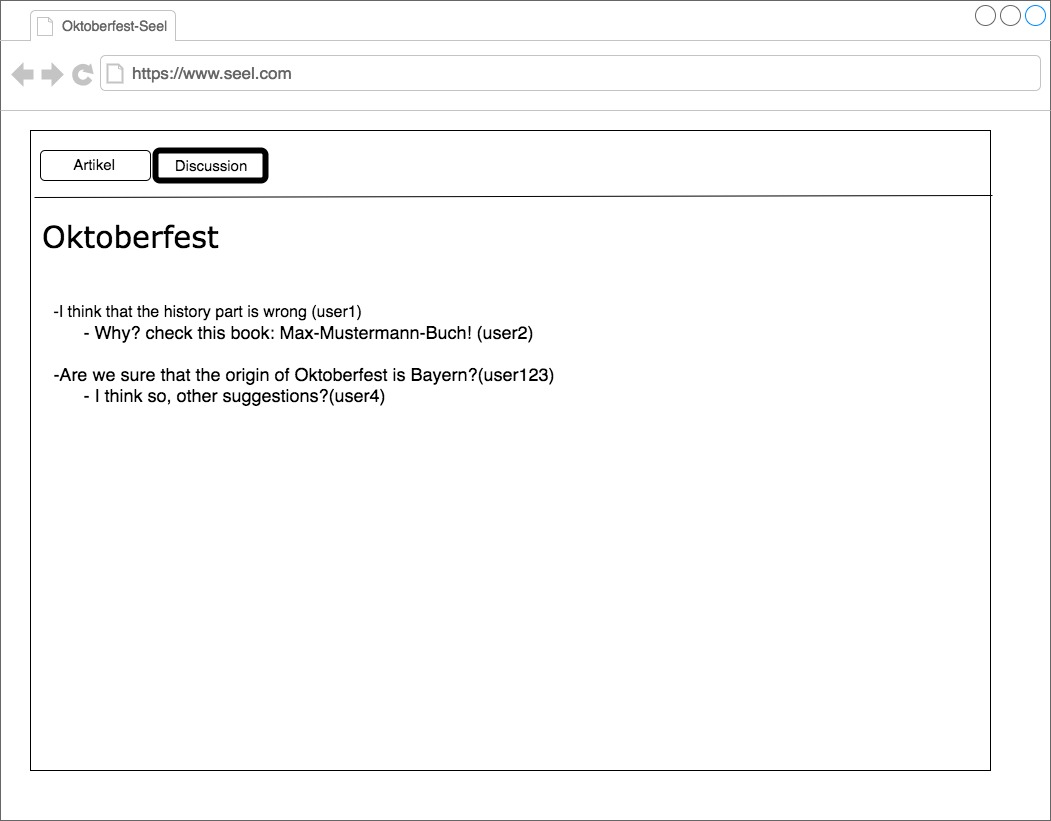
\includegraphics[width=0.6\textwidth]{Pictures/discussion1.jpg}
    \caption{Discussion page example}
\end{figure} 

\subsection{Benefits}
The main idea behind discussion pages is to allow the users to discuss about a specific article in the Wiki.
Topics written by users tend often to start discussions, mostly because the authors aren’t professionals in the specific fields they write about. To avoid having multiple wiki articles about one Subject as a result of different opinions, we would allow and recommend user to discuss one article in purpose of reaching a common opinion about the subject.

\subsection{Types of discussion pages}
\begin{itemize}
\item Discussion regarding user-generated articles
\item Discussion regarding BSI page: unlike user-generated articles discussion pages, these discussion pages are not aiming to improve the content of BSI pages, but just to discuss the topics and share question regarding them.
\item Discussion regarding FAQ: This page will be used to enable the users of our platform to ask general questions regarding the usability of this page which was not found in the FAQ.
 
 \end{itemize}
 
\section{Information page - Priority: MEDIUM}
 The Information page allows EVERY guest to share and publish general questions to the community in our platform.\\
 Since the platform main concept is to share the BSI pages and good content through Wiki to the community, we came upon a conclusion to keep it "hidden" and just link it in the FAQ page (See graphic below). \\
 
 \begin{figure}[h] 
    \centering
    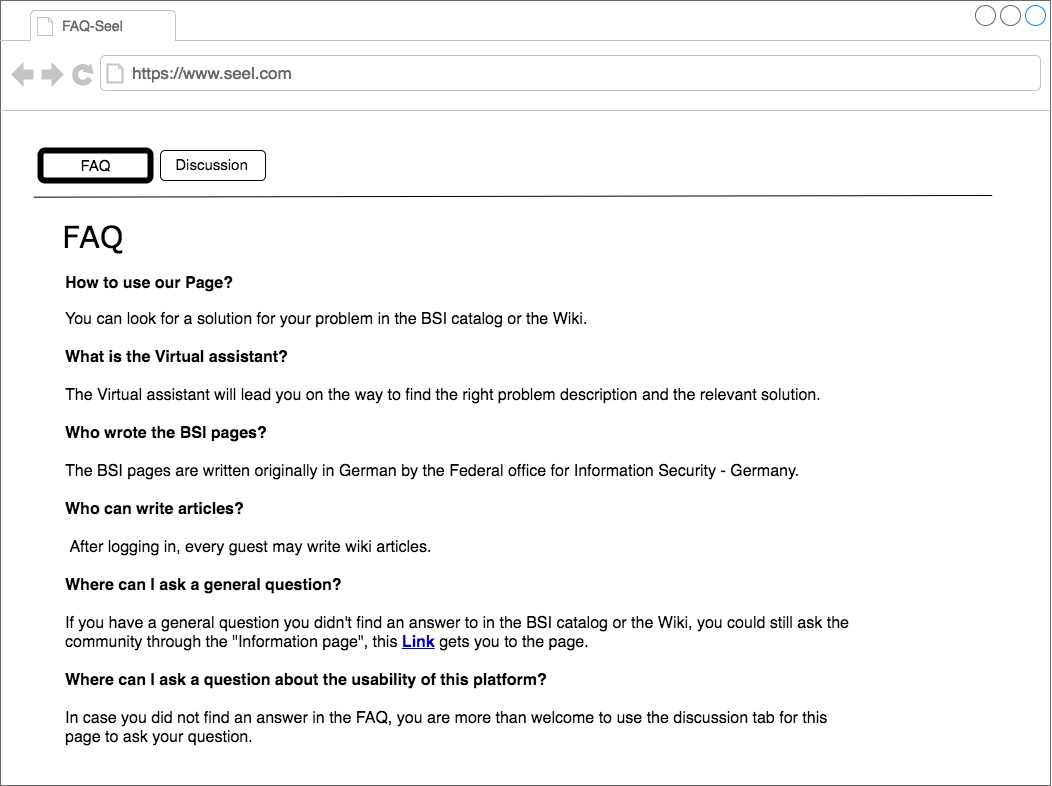
\includegraphics[width=0.6\textwidth]{Pictures/information1.jpg}
    \caption{Link to the Information page in the FAQ}
\end{figure} 

The Information page should allow every guest to write content, so unlike normal articles, there should be a text field on the top of the article, provided with a submit button.

\begin{figure}[h] 
    \centering
    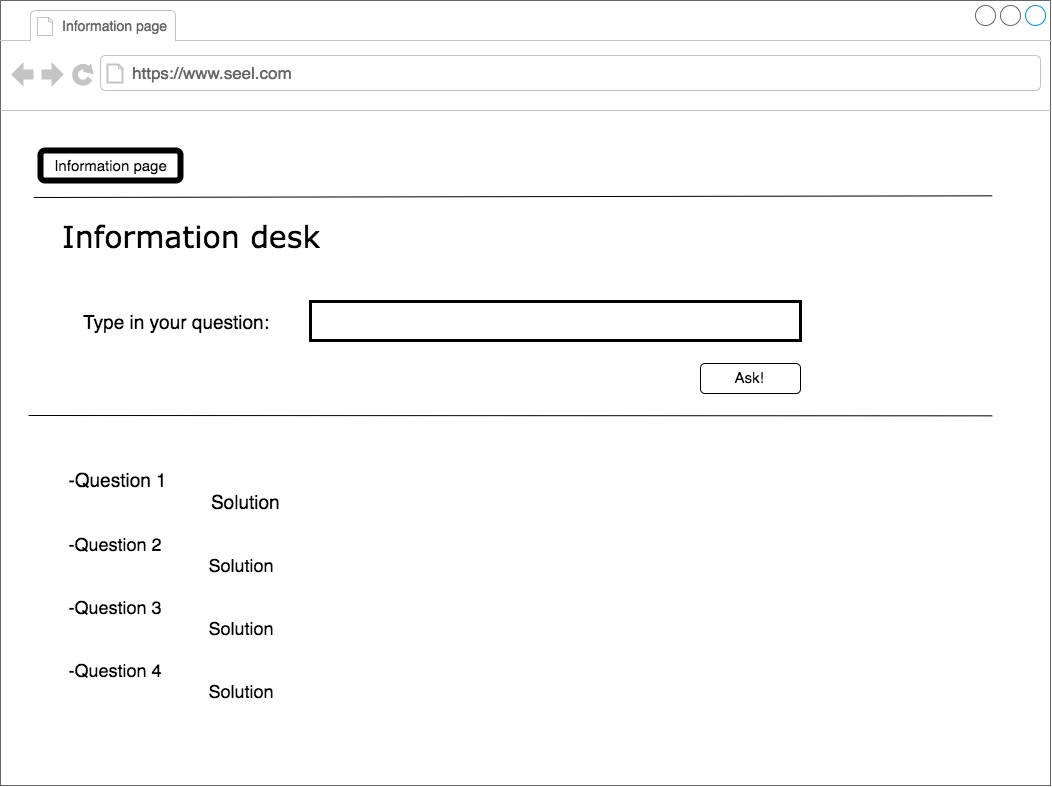
\includegraphics[width=0.6\textwidth]{Pictures/information2.jpg}
    \caption{Information page structure}
\end{figure} 

\section{Report a Mistake  - Priority: MEDIUM}

Since the BSI pages are automatically translated, translation errors may occur quite often, and since the users can't update the pages and correct the mistakes themselves, we need a tool, in which users can inform the mods in case they find an error. \\
The page consists of a text field, in which the users are asked to fill in information regarding the mistake they found.\\
The field can't be empty, but the users are free to write description and improvement tips as they want.

\begin{figure}[h] 
    \centering
    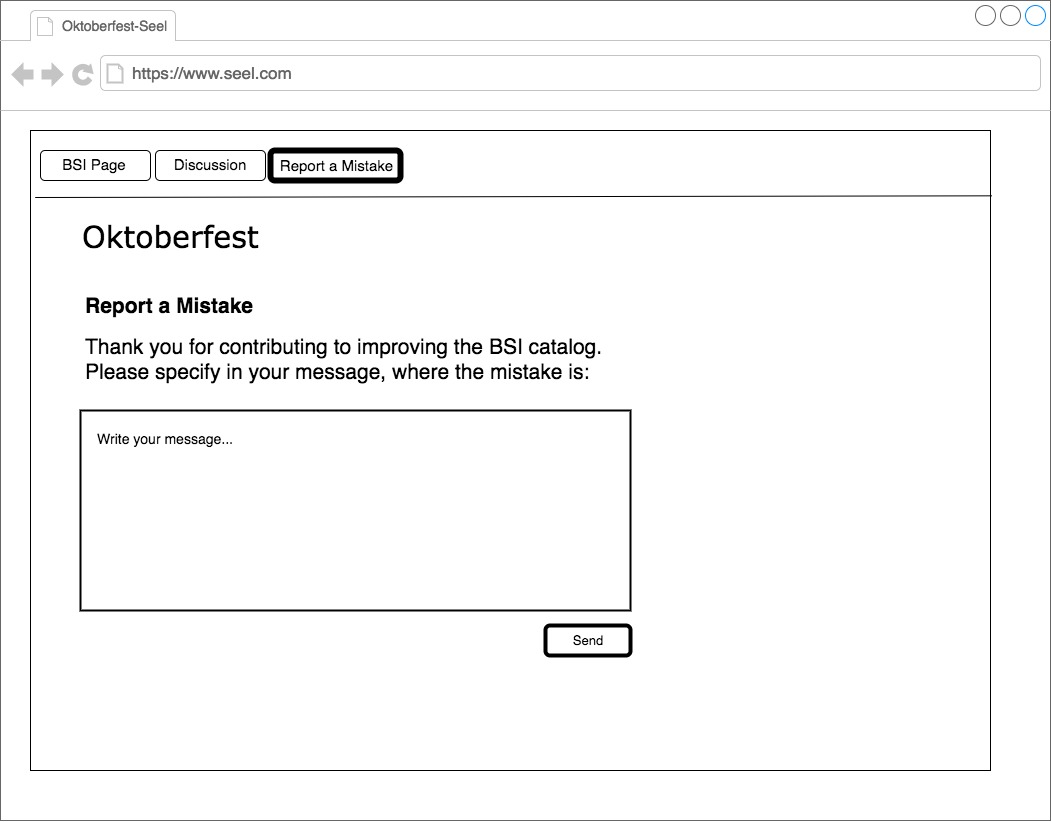
\includegraphics[width=0.6\textwidth]{Pictures/report1.jpg}
    \caption{The structure of "Report a Mistake}
\end{figure} 

The moderators should check these forms and, if necessary, correct the errors.


\section{Labels - Priority: HIGH}
 
\begin{tcolorbox}[breakable,colback=red!14,colframe=red!40!black,title=UPDATE 30/11/2017]
Labels should inform website users about the current state of content. 
\\
Types of labels:
\begin{itemize}
    \item \textbf{creation status}: an automatically generated label which gives information about how long ago the content has been created. Formatting in hours, weeks, months and years.
    \item \textbf{unchecked/checked}:The default is unchecked, content read by moderators and where the content is appropriate will get a checked label. When a user edits a checked article, it will be automatically gets a unchecked label. 
    \item \textbf{helpful label}: For a certain number of upvotes, content should get a helpful label. This should be scalable
    \item \textbf{content type}: use labels as a 'path'/show where the page is: news, archive, BSIc. Several content types are possible.
    \item \textbf{important}: The important label is mainly to draw attention to certain news.
\end{itemize}

It should be possible to label each content, articles as well as news. For the news it should be possible to put a label within an article. For example, to mark individual news with an important label. It should be possible for the admin to create a new label that he considers appropriate.


\end{tcolorbox}

Here are some examples for label
\begin{figure}[h] 
    \centering
    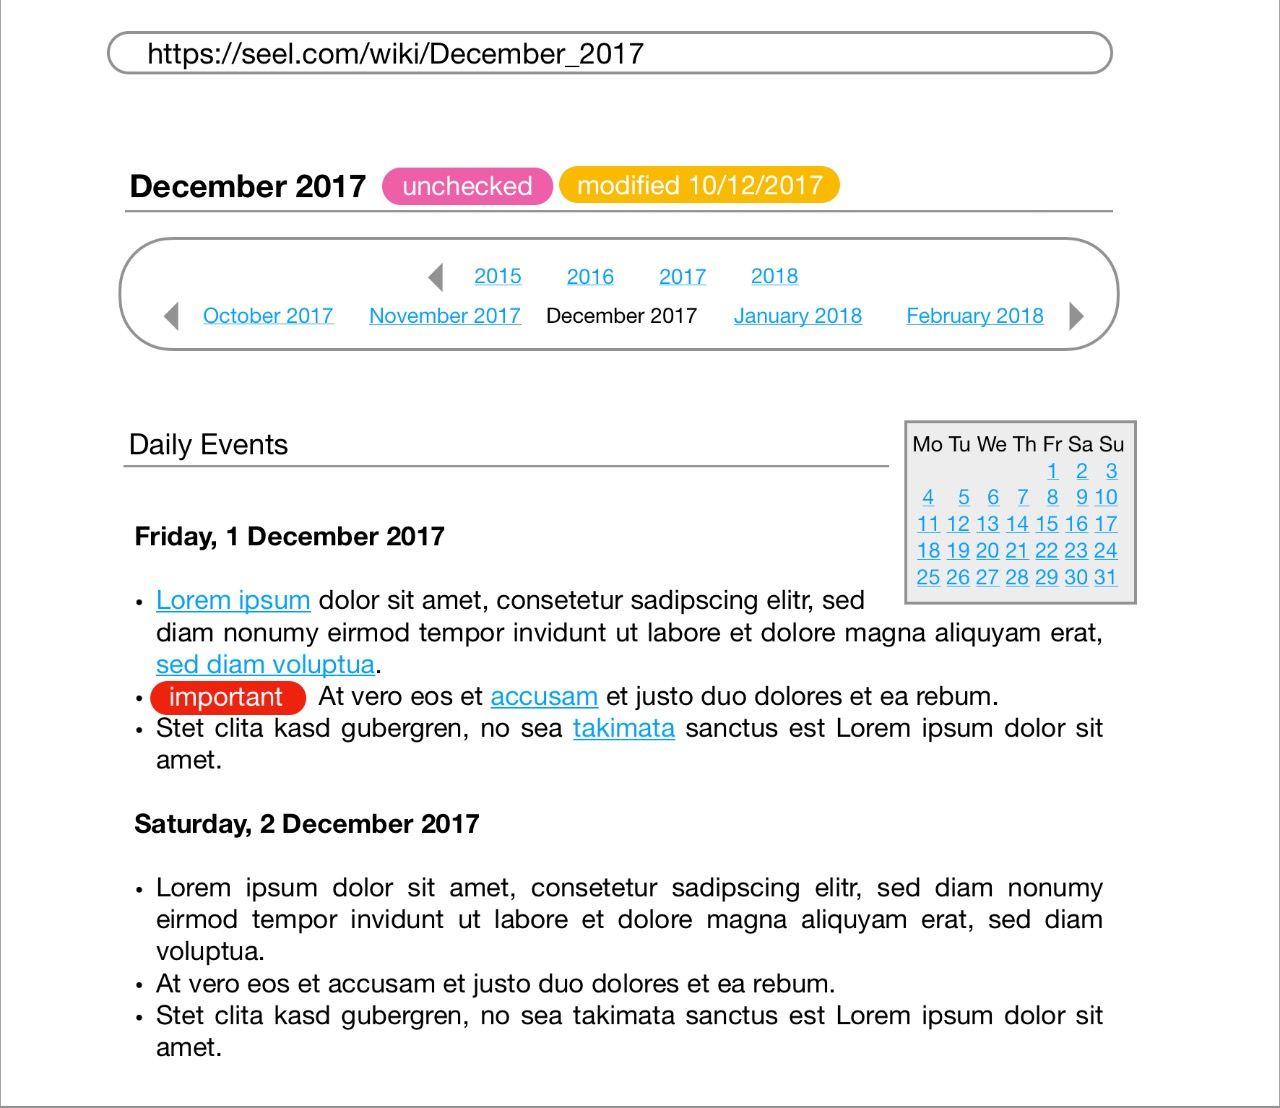
\includegraphics[scale=0.25]{Pictures/labels}
    \caption{Labels in the News section}
\end{figure} 


\section{Up/Down Votes - Priority: MEDIUM}
\begin{tcolorbox}[breakable,colback=red!14,colframe=red!40!black,title=UPDATE 30/11/2017]
Article votes would be nice in form of a “Is this page helpful?” Question with yes/no buttons at the end of it, which could generate after 100 yes votes a label “Helpful” or through many no votes draw the attention to revisions the article.
Every website user can vote, including the guest. When an article is re-linked during an update, all the votes will remain.
\end{tcolorbox}

\begin{figure}[h] 
    \centering
    
\includegraphics[width=0.6\textwidth]{Pictures/helpful_vote}
    \caption{Microsoft helpful-vote example}
\end{figure} 

\section{Reputation Points (Karma Points) - Priority: MEDIUM}
\begin{tcolorbox}[breakable,colback=red!14,colframe=red!40!black,title=UPDATE 30/11/2017]
Reputation points should motivate users to get involved on the side and reward them for that.\\
\end{tcolorbox}

\begin{figure}[h] 
    \centering
    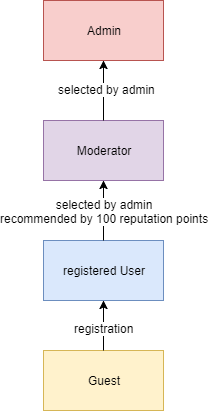
\includegraphics[scale=0.6]{Pictures/UserStructure}
    \caption{Waffle label analyse}
\end{figure} 


\begin{tcolorbox}[breakable,colback=red!14,colframe=red!40!black,title=UPDATE 30/11/2017]
We would like to keep a similiar (best-practice) user structure to Wikipedia. In our system we will have admins, the “sichter” will be our “moderator”, we will also have registered user and guests. \\
However after intensive discussion about how Karma (or reputation points) is generated, we decided to just keep the “article upvoting” generated votes for an article only without passing it to the user, since the quality of writing / editing, perhaps only a few, article isn’t representative of the trustworthiness of a user.\\
Only users which have had a big number (100) of approved edits/writings are recommended to the admin as a new mod. However it remains the decision of the admin whom appoint as mod. 
If the admin needs help he can select a mod and add him as as additional admin.
\end{tcolorbox}


\section{User Access to BSI Catalogue Pages - Priority: HIGH}
\label{2nd_bsi_link}
While the general access to alter the pages of the BSI catalogue should be restrictive (see section~\ref{BSIc}) users who write an article should still be allowed to link their article in the pages of the BSI catalogue.

\begin{tcolorbox}[breakable,colback=red!12,colframe=red!40!black,title=UPDATE 15/11/2017]
    For mockups of the linking process detailled here see Appendix~\ref{appendix_bsi_link}.
    After or while users write their articles they are presented with the option to link it to the BSI catalogue.
    This option leads users to another page. Here:
    \begin{itemize}
            \begin{comment}
        \item on their first visit, users are presented with 
            \end{comment} 
        \item users can search for wiki content they want to link to,
        \item users can directly browse the BSI tree to find the page they want to link to,
        \item on the left  users see a list of titles of wiki pages that they already have linked their article to
            .
    \end{itemize}
    There is no restriction on the number of pages an article can be linked to.
    So the list of linked pages should offer a scroll bar if the list exceeds the page limits.
    If users click on a search result, a BSI tree item or an item of the list of linked to wiki pages they are brought to the page in question.
    There, if users want to link to a word they click on/mark the word they want to link their article to.
    Alternatively, they click on/mark the ``See also'' section of the page.
    Both times the selection has to be confirmed and brings the user back to the second page which features the list of linked pages.
    The list of search results should be limited to ten.
    So that, users have to change or add to his keywords if they did not get the page they were looking for.
    All pages should have a ``Back'' or ``Cancel'' button.  
\end{tcolorbox}


\section{Automatically created best 10 Suggestions when linking to BSI - Priority: LOW}
\begin{tcolorbox}[breakable,colback=red!18,colframe=red!40!black,title=UPDATE 01/12/2017]
   For mockups of the linking process detailled here see Appendix~\ref{appendix_bsi_link}.
   The best 10 Suggestions are nice to have but low periorized. It would be nice if these suggestions appear automatically after writing an article. Our idea was that these suggestions would be found through the internal search. These suggestions are always updated when the user enters something again in the search field. This topic is low-periodized and does not need to be strongly considered.   
\end{tcolorbox}



\section{Extended Wizard (Work in Progress) - Priority: LOW}

